\newcommand{\RNum}[1]{\uppercase\expandafter{\romannumeral #1\relax}}

\section{Study overview}
The dissertation is based on data from two learning experiments, referred to as Study 1 and Study 2. Each of these experiments has resulted in multiple articles, some published in journals, others as preprints, or included as additional analyses in this dissertation. 

Study \RNum{1} was designed to test whether frequent task switching can enhance learning. This experiment spanned eight days, starting with a baseline test on day one, followed by three days of training intervention. This training intervention contrasted two training groups learning to pump on flat slopes in slalom: an interleaved training group, which practiced pumping on three slalom courses each day in interleaved order (ensuring skiers never repeated the same slope consecutively), and a blocked training group, which practiced pumping on one slalom course each day (with the order counterbalanced across skiers). After the training period, the skiers had a three-day break without skiing. On the third day, they completed a retention test. This study resulted in Paper \RNum{1}, which reports the learning effects between the two learning groups. Additionally, we collected positional data from the skiers using a local positioning system during the baseline and retention to study the kinematic changes due to the intervention. This analysis is reported in Paper \RNum{2}. 

\begin{figure}
    \centering
    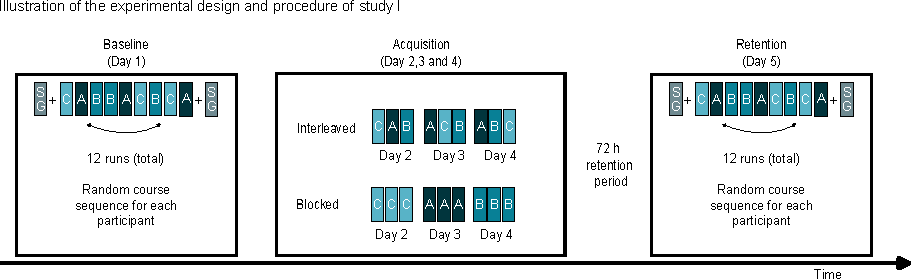
\includegraphics[width=1\linewidth]{figure/figure_methods_CIdesign.pdf}
    \caption{Enter Caption}
    \label{fig: ci_illustration}
\end{figure}


Study \RNum{2} was designed to identify the most effective teaching signal for helping skilled performers learn strategy selection to enhance performance. This learning experiment spanned three days, beginning with a baseline test on day 1. This baseline test was followed by a training intervention (acquisition) consisting of three training sessions. The intervention contrasted reinforcement learning with two supervised learning groups as teaching signals. In the reinforcement learning group, the skiers learned to select optimal strategies by seeing their times to inform their next strategy choice. Conversely, in the supervised learning groups, the coaches selected strategies for the skiers. In the supervised (target skill) learning group, we educated experienced coaches on the theoretically optimal strategy and instructed them to select this strategy for the skiers and give them feedback on this strategy after every trial. In the supervised (free choice) learning group, we recruited two coaches from each group of the tested ski teams to select a strategy that they believed would make the skier faster. Before allowing the skiers (reinforcement learning) or the coaches (supervised learning) to freely choose strategies, we conducted a forced exploration session where all participants tested every strategy. On day 3, the skiers performed a retention test and a transfer test, independently select strategies. This study resulted in Paper \RNum{3}, which reports the learning effects of the two teaching signals on strategy selection. Additionally, we used data from the forced exploration session to analyze and estimate which strategies yielded the best performance for the skiers. Denne analysen er også gjort Paper\RNum{3}, men vi har gjort en ekstra analyse som vi har rapportert her. 
\begin{figure}[H]
\centering
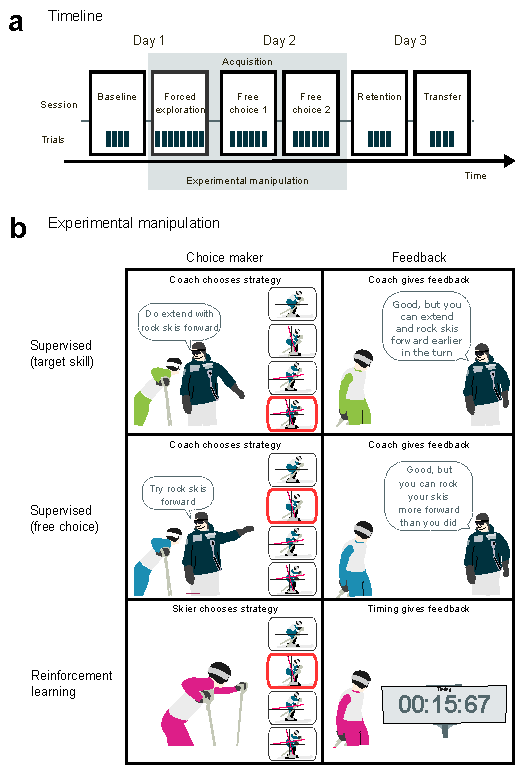
\includegraphics{figure_method_experiment.pdf}
\caption{Acceleration in the local positioning system section.\textbf{a.} Estimated acceleration during baseline and retention for the local positioning section. \textbf{b}. Expected mean difference between baseline and retention in the local positioning section.\textbf{c.} Estimated total gate-to-gate acceleration during baseline and retention in the local positioning section. \textbf{d}. Expected mean difference between baseline and retention in the local positioning section. The black lines denote the expected mean or differences in mean, with the shaded area representing their 95\% credible interval (CI). Each gray point or line represents one run trial by a skier}\label{fig: acc}
\end{figure}


\section{Setup}
All studies were conducted in the indoor ski hall, SNØ, located in Oslo, Norway (\url{https://snooslo.no/}). In this ski hall, we used the upper part of the race hill, which is a long flat section with two small rollers. The snow of this flat section was watered before testing each group of skiers to ensure uniform and fair conditions for all skiers. 

\begin{figure}
    \centering
    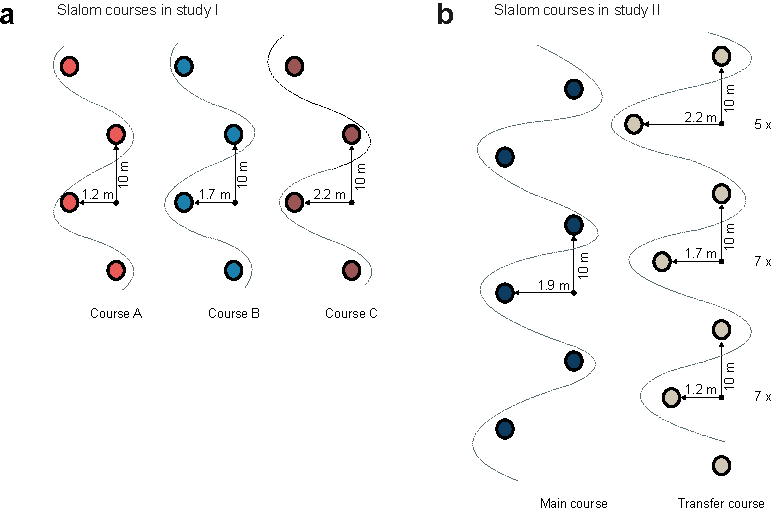
\includegraphics[width=1\linewidth]{figure/figure_methods_courses2.pdf}
    \caption{Enter Caption}
    \label{fig:enter-label}
\end{figure}

In study \RNum{1}, we set up three slalom courses to test the contextual interference effect. These courses required skiers to execute pumping movements with different timings and amplitudes for effective performance. All three courses had a vertical gate distance of 10 meters due to space constraints, forcing parallel setup. However, the courses had varying offsets: 1.2 meters for Course A, 1.7 meters for Course B, and 2.2 meters for Course C. These specific gate offsets were chosen to create diverse pumping demands without making it impossible to pump. Fig. 

In study 2, we set up two slalom courses to test. The main slalom course was used in all sessions except the transfer test and featured a 10-meter distance and a 1.9-meter offset. The transfer test assessed skiers' ability to transfer learning to a more realistic alpine race course. This test course included a progression in gate offset: five gates at 2.2 meters, seven gates at 1.7 meters, and seven gates at 1.2 meters. 

In both studies, we used stubbies (short gates) instead of long gates to minimize energy dissipation upon hitting the gate\cite{minetti_biomechanics_2018}. Using stubbies allowed skiers to focus better on skill execution of the strategy without the distraction of clearing the gate, which could hinder learning. In addition, this approach minimized hole creation that occurs when a long gate is forcefully slammed into the ground. 

We adopted the same standardized start procedure in both studies. The involved setting the start gate 20 meters before the first gate. Here, skiers were instructed to place their toe bindings behind the starting gate. Upon receiving the clearance signal, skiers were to place their skis parallel, lift the poles from the ground, and glide out of the start gate without using poling or skating to generate propulsion. Timing was recorded using a wireless photocell timing system (HC Timing wiNode and wiTimer; Oslo, Norway), starting when the skier crossed the first photocell pair situated 10 meters below the starting gate. (See https://osf.io/9numq for a supplementary video illustrating the starting procedure and setup).


\section{Participants}
Our target population for making inferential claims was skilled alpine skiers worldwide. Therefore, we recruited only skiers aged 15 and older, marking the entry age for participating in Federation Internationale de Ski (FIS) races. We chose skiers aged 15 years and older to ensure that they could handle the icy snow conditions we prepared in the ski hall and had the basic skills necessary to learn the strategies we developed. Beyond these criteria, we deliberately recruited skiers with diverse skill levels—from skilled junior ski academy skiers to Olympic skiers—to enhance the generalizability of our findings.

Our sample size approach in both studies was to recruit as many skiers as possible during the available testing window, and was justified by the 'resource constraints' and the 'whole population' criteria \cite{lakens_sample_2022}. First, the relatively small and geographically dispersed population of skilled alpine skiers limits the number of available participants.  Second, coaches and skiers must be willing to participate in the intervention. For coaches and skiers at this level to show this willingness, they must be convinced that the intervention will benefit the skiers' development, as it typically replaces the skiers' regular training due to their already high training volumes. Finally, the narrow testing window, typically in the spring and summer, coincides with the indoor skiing training periods for many ski teams, leading to a high demand for training lanes. These combined factors make it challenging to recruit a large number of participants and to reach a specific benchmark.  

In Study 1, we successfully recruited 66 skilled alpine skiers (31 females) from Norway, with a mean age of 17 years (SD = 2.7). Of these, 51 skiers attended ski academies and had either already earned International Ski Federation (FIS) points or were about to do so in the upcoming season. Twelve skiers competed at the club level in age-specific categories for those aged 14 to 16 (but with the necessary skill level), while three skiers were elite skiers outside the national team preparing for the next season. Unfortunately, due to COVID-19, 12 of these 66 skiers were quarantined and unable to participate in the retention session. We did not ask the first groups of the tested ski teams to report their FIS points on slalom, resulting in a lack of FIS points and world ranking data for these skiers. 

Study 2 involved a smaller sample (n=18) from the larger pool of skiers in Study 1 (n=66), where we recorded the skiers' positions using a local positioning system in the upper section of the course. The smaller sample included 18 alpine skiers (mean age = 16.7 years, SD = 1.1; 7 females, 11 males) from three ski academies. Except for three skiers, all participants had previously competed in FIS races, with recorded FIS points in slalom (M = 115, SD = 31). However, these FIS points may not accurately reflect their skill levels due to the pandemic-related challenges in organizing races, which limited opportunities to accumulate points.

In Study 3, we successfully recruited 98 alpine skiers from Norway and Sweden (mean age = 18.1 years, SD = 2; 40 females, 58 males). Two skiers were excluded from the analysis due to injury prior to the study (n=1) or sickness (n=1), resulting in 96 skiers who completed the study and were included in the analysis. The tested groups of skiers included five ski academies, three senior development teams, and two national ski teams. The skiers were generally highly skilled, with mean FIS points in slalom 55.4 (SD=32). Their median world rank was 605, though there was considerable variability (Q1 = 248, Q3 = 1390.5). A smaller subset of skiers (n = 13) were not world-ranked, as they had yet to compete in internationally sanctioned races necessary for calculating FIS points and rankings. Before data collection for this study, we set the minimum sample size to 80 skiers, which we deemed appropriate for this context. Prior to data collection, we conducted power simulations for sample sizes of 80, 100, and 120 skiers. These simulations revealed powers of 0.60, 0.75, and 0.80, respectively, for the smallest effect size of interest (0.3 second difference between groups) (\url{https://osf.io/c4t28}). 


\section{Design and procedure}

\subsection{Study 1}
In Study 1, we employed a between-subjects design and allocated skiers to either a blocked or interleaved learning group. The experiment began with a baseline test consisting of nine trials (three trials on each of courses A, B, and C), where skiers skied as quickly as possible without receiving time feedback. The trials in these courses were distributed randomly to each skier under the condition that the skier did not perform two consecutive runs on the same course. In addition, the skiers performed a straight gliding task on a dedicated lane before, midway (randomly assigned), and after the nine trials.

After the baseline test, we used a randomized-blocked design to allocate skiers into either the blocked or interleaved learning group based on their baseline test times. Specifically, we extracted each skier's best run from the baseline on each course and divided it by the average of the straight gliding runs from the baseline. Skiers were then ranked from fastest to slowest and paired in ascending order, and each consecutive pair was randomly assigned to either the interleaved or blocked group.

Immediately after the baseline test on day one, skiers attended a workshop where we explained the mechanical principles of the pumping technique and presented quantitative evidence supporting this strategy. Skiers then completed three training sessions over three days, with each session including 15 runs: 12 runs on the three courses and three straight-gliding runs. The interleaved group skied all three courses each day in a randomized interleaved order, ensuring no more than two consecutive runs on the same course. The blocked group performed all their runs on one course (A, B, or C) per day, with the course order counterbalanced across participants. 

Three days (72 hours) after the last training session, the skiers returned for a retention test, consisting of 12 runs (three runs on each of the three slalom courses and three straight-gliding runs). The order of the runs in the courses was scheduled in a semirandom order, with the condition that no more than two consecutive runs could be performed in the same course. As in the baseline test, the skiers performed a straight gliding task on a dedicated lane before, midway (randomly assigned), and after the nine trials. The skiers were instructed to ski as fast as possible but did not receive any performance feedback during the posttest. This design allowed us to compare the effects of blocked versus interleaved practices on the learning and performance of the pumping strategy. 


 \subsection{Study 2}
In Study 2, we employed a between-subjects design and framed the task of learning to choose effective strategies as a multiarmed bandit problem\cite{sutton_reinforcement_2018} (see the methods section in Paper 3 for a detailed description). Here, the options (or bandits) that the skiers needed to learn and select to ski as quickly as possible were the four technical strategies detailed in section \ref{introduction: strategies}.

To determine which teaching signals most effectively drive this learning process, we allocated skiers into one of three learning groups. In the supervised (target skill) learning group, the skiers were instructed by a coach to choose the theoretically best strategy (that is, extend with rock skis forward) and received feedback on their execution of this strategy after every trial. For this learning group, we engaged highly experienced ski coaches to ensure credibility in promoting this strategy, and these coaches were educated by us before the data collection. To the skiers, these coaches told that the 'extend with rock skis forward’ strategy was the most effective strategy for skiing fast on flat terrain in slalom, citing theory and quantitive evidence from research literature in alpine skiing mechanics \cite{reid_kinematic_2010, mote_accelerations_1983, lind_physics_2013, lemaster_skiers_1999, lemaster_ultimate_2010}. In the supervised (free choice) learning group, the skiers were assigned to one of two coaches selected from the ski team undergoing testing. These coaches were instructed to maximize their assigned group of skiers' performance in the slalom course by choosing one of the four strategies for each trial. Although the coaches in these two supervised learning groups had access to the skiers’ data after each trial, they were not allowed to share the times with the skiers. In contrast, the reinforcement learning group learned the value of these strategies themselves by observing the times for a chosen strategy after every trial to guide their strategy choices, with the aim to select the best strategy. This group was not assigned a coach but a person to communicate with the skiers, record their choices, and encourage them to ski quickly to prevent boredom effects. See the original paper for more information.

Læringseksperimentet begynte med en baseline som bestod av fire runder i slalåmløypen (main course in fig), pluss en straightgliding runde der utøverne kjørte rett ned løypeseksjonen i en egen dedikert bane for dette. Før utøverne gjennomførte disse fire rundene og straight glidingen gjennomførte de to oppvarmingsrunde: en gjennomført som frikjøring og som gjennomført som oppvarming i løypen, der de fikk instruksjoner og tilbakemelding på utførelsen av startprosedyren. 

Etter dette allokerte vi utøverne i tre læringsgrupper supervised (target skill) learning, supervised (free choice) learning and reinforcement learning. For denne oppgaven brukte vi en randomisert blocked approach for å ta hensyn til preeksisterende forskjeller mellom utøvere. Specifically, we computed each skier’s average across the four trials at baseline and ranked them accordingly. We then created \textit{n} blocks with block sizes corresponding to our three learning groups for the entire list of skiers and assigned these skiers to these predefined blocks. Finally, we randomly allocated the skiers to the different learning groups within each block (Fig. \ref{fig:experiment}b). I mellomtiden hadde utøverne en pause på 60 minutter i varm sone. 

The learning groups participated in sessions at different times to prevent treatment
diffusion \cite{maxwell_designing_2017}. Since the ski group consisted of teams that regularly trained and lived together during data collection, they were instructed to keep session information private. To complete the learning experiment within the ski hall's opening hours, the two supervised learning groups underwent training simultaneously. We arranged coach stations in the finishing area with space and vision dividers to prevent information leakage between coaches. Additionally, a Python script was used to fetch race times from the timing system, which were filtered for each coach and transmitted to the respective station so that each coach could only see their own skiers' times. The learning group that begun traing after the learning group assignment (reinforcement learning versus supervised learning) was randomized and counterbalanced across the ski teams tested. 

During the first session following the learning group assignment, we engaged the skiers in forced exploration. We gathered the skiers within each learning group and began by introducing them to the four strategies identified to enhance racing times on flat slopes in slalom. Each strategy was detailed with illustrative drawings and word explanations, as outlined in (SJEKK). To ensure understanding, skiers participated in two short familiarization trials for each strategy or continued until their execution met our standards.

After reviewing the strategies, we asked the skiers and the coaches in the supervised (free choice) learning group to rank the strategies (1=best; 4=worst) based on their perceived effectiveness in improving race times on flat sections of a slalom course. We explicitly instructed the coaches and skiers not to discuss the strategies with each other during the instruction and ranking process. Notably, the same instructor conducted all learning sessions within the tested ski group.

Following this review, the skiers performed eight trials on the slalom course, testing all strategies with two trials per strategy. Strategies were randomly assigned, ensuring that the first and last four trials included all strategies. During this session, the reinforcement learning group received feedback on their timing, while the coach provided feedback in the supervised learning groups.

 






















The first session following the learning group assignment was forced exploration. In this session, we gathered the skiers within each learning group and began by introducing them to the strategies. We explained that we had identified four strategies to enhance racing times on flat slopes in slalom. Each strategy was then detailed, supported by illustrative drawings in Fig. \ref{fig: strategies}) and corresponding word explanations as outlined in (SJEKK). To confirm the skiers had understood the strategies, we conducted two short familiarization trials for each strategy or until the skiers' execution met our strategy execution standards. After reviewing the strategies, we asked the skiers and the coaches in supervised (free choice) learning groip to rank the strategies (1=best; 4=worst) based on what they believed would best improve race times in the flat section of a slalom course. During the instruction and ranking process, the coaches and skiers were explicitly instructed not to discuss the strategies with each other. Notably, the same instructor was used for all learning groups within the tested ski group. After this review, the skiers performed eight trials in the slalom course where they tested all strategies (two trials for each strategy). These strategies were randomly assigned to each skier under the condition that the first and last four trials included all strateiges. During this session, the reinforcement learning group received feedback on their timing, whereas the coach provided feedback in the supervised learning groups.

 



























The first session after learning group assignment involved a forced exploration.
Here, skiers within the learning group were gathered, and the session started by intro-
ducing them to the strategies. We explained that we had identified four strategies to
enhance racing times on flat slopes in slalom. Subsequently, each strategy was detailed,
supported by illustrative drawings in 1b Figure and corresponding word explanations
as outlined in the Supplementary A. To confirm comprehension, we conducted two
short familiarization trials for each strategy or until the execution met our performance
standards. After reviewing the strategies with the skiers, we gathered them in their
respective learning group and asked them to rank the strategies (1=best; 4=worst) for
what they believe to be the best strategies for improving race times in the flat section
of a slalom course. Throughout the instruction and ranking process, skiers were explic-
itly instructed not to discuss the strategies with each other. It is important to note that
the same instructor was used for all learning groups within the tested ski group. After
this, the skiers conducted a total of eight trials on the course, with two trials for each
strategy. Here, we handled the practice order effect probabilistically by randomizing
the order for each skier, under the condition that the first and last four trials tested
all strategies. During these trials, the reinforcement learning group received feedback on the timing, whereas the coach provided feedback in the supervised learning groups


\section{Measures and analysis}
De ulike målene og forskningspørsmålet har favnet nokså bredt. Derfor har jeg valgt å dele inn measures og analyse etter hva som er formålet med de enkelte studiene. 


\subsection{Paper 2}
I Paper \RNum{2} var målet å forsøke å forklare forbedringer i renntidene fra Studie \RNum{1}. For å få innsikt i dette monitored vi skiers using a local positioning system in a five gate long section in the middle of the course during the baseline and retention sessions. Opprinnelig var det opprinnelige opptaksområder betydelige lenger, men på grunn av utfordringer med data kvaliteten i det øverste området av sekvensen (der nodene kom for tett på veggene i skihallen) måtte vi korte ned området. 




\subsection{Paper 3}
In Paper \RNum{3} (basert på Studie \RNum{2}) ønsket vi å teste om reinforcement learning forbedret sine renntider mer under trening (acquisition) og presterte bedre under retention og transfer enn supervised (free choice) learning, men også å sammenligne opp mot supervised (target skill) learning som var på benchmark gruppe for optimal prestasjon gjennom optimale valg av strategier. To account for these multilevel data structures, we leveraged linear mixed-effects models. To model random effects, we adopted a design-driven approach \cite{barr_random_2013, barr_learning_2021}, where we sought to account for all nonindependence introduced by repeated sampling from the same ski group and skier. We deployed classical frequentist statistics and fitted these models with the lme4 package \cite{bates_fitting_2015} in the R \cite{r_core_team_r_2022} programming language. We used a simple coding scheme for our predictors where the intercepts represent the estimated mean of the cell means and the contrasts represent the estimated difference with respect to the reference level, which we set for reinforcement learning. Two-tailed p values and degrees of freedom for each model were derived using the lmerTest package \cite{kuznetsova_lmertest_2017} via the Satterthwaite approximation method. Alpha was set to 0.05 for all test statistics.




These race times were analyzed using linear mixed-effect regression models. Initially, we planned to normalize the racing times by expressing the racing times as the difference from the straight-gliding time performed at the beginning of every session (like we did in Study \RNum{1}). However, practical considerations led us to deviate from this approach. This change was necessary because we had to flip or shift the course after each day to ensure snow conditions with the least damage. Unfortunately, these adjustments made maintaining a clean, straight-gliding lane difficult since the straight gliding lane crossed many areas with damage to the snow surface (holes) from the previous course set (see Supplementary Methods C for an image of these holes). Collisions with these holes affected the race time, adding noise to the results. Therefore, we used a more conservative approach and analyzed the raw racing times instead of analyzing the normalized racing times.

For the acquisition session, we modeled race time using Session (forced exploration, free choice 1, free choice 2) and Learning group (reinforcement learning, supervised: free choice learning, supervised: target skill learning), and their interactions, as predictors. For retention and transfer, we modeled race times at these sessions, with learning group added as a predictor. In addition, we used the average performance for each skier on the baseline test as a predictor to improve estimate precision and adjust for any group differences at baseline testing. 

To model the effect and development of the strategies we broke the analysis up into different sub-models. One analysis focused on differences in the strategies and groups regarding Forced Exploration, where all participants had completed all strategies. Another analysis examined the transition from Forced Exploration to retention for both supervised (free choice) and reinforcement learning. The final model investigated the development between groups specifically for the "extend with rock skis forward" strategy. Session was coded as a continuous variable in all models. 

I artikkelen har vi også forsøkt å forklare disse tidene, men har valgt å ikke presentere disse analysene i denne thesis og dermed også ikke presentert dem her. 










Due to the hierarchical structure of the data, our general statistical strategy relies on multilevel modeling. At the first level, each skier performed multiple trials during each session. At the second level, each skier was nested within groups of ski teams that performed the experiment together. To account for these multilevel data structures, we leveraged linear mixed-effects models. To model random effects, we adopted a design-driven approach \cite{barr_random_2013, barr_learning_2021}, where we sought to account for all nonindependence introduced by repeated sampling from the same ski group and skier. We deployed classical frequentist statistics and fitted these models with the lme4 package \cite{bates_fitting_2015} in the R \cite{r_core_team_r_2022} programming language. We used a simple coding scheme for our predictors where the intercepts represent the estimated mean of the cell means and the contrasts represent the estimated difference with respect to the reference level, which we set for reinforcement learning. Two-tailed p values and degrees of freedom for each model were derived using the lmerTest package \cite{kuznetsova_lmertest_2017} via the Satterthwaite approximation method. Alpha was set to 0.05 for all test statistics.




























